\section{Paper Reading: CDL}

\begin{frame}{Weakly Supervised Fine-grained Image Classification via Correlation-guided Discriminative Learning}
    \begin{itemize}
        \item \textbf{Author:} Zhihui Wang, Shijie Wang, Pengbo Zhang...\footnote{大连理工大学王智慧教授、李豪杰教授、王世杰博士等}
        \item \textbf{Keywords:} Fine-grained Image Classification; Discriminative Region Grouping; Discriminative Feature Strengthening
        \footnote{细粒度图像分类,判别区域分组,判别特征增强}
        \item \textbf{Contribution:} \textbf{Propose} an end-to-end Correlation-guided Discriminative Learning (CDL) model to fully mine and exploit the discriminative potentials of correlations for WFGIC globally and locally. 
        \footnote{提出了一个端到端相关性引导判别学习(CDL)模型,以充分挖掘和利用相关性在全局和局部的鉴别潜力。}
        % \item 开源代码:无
    \end{itemize}
\end{frame}

\begin{frame}{Motivation for correlation-guided discriminative learning}
    \begin{figure}[htb]
        \centering
        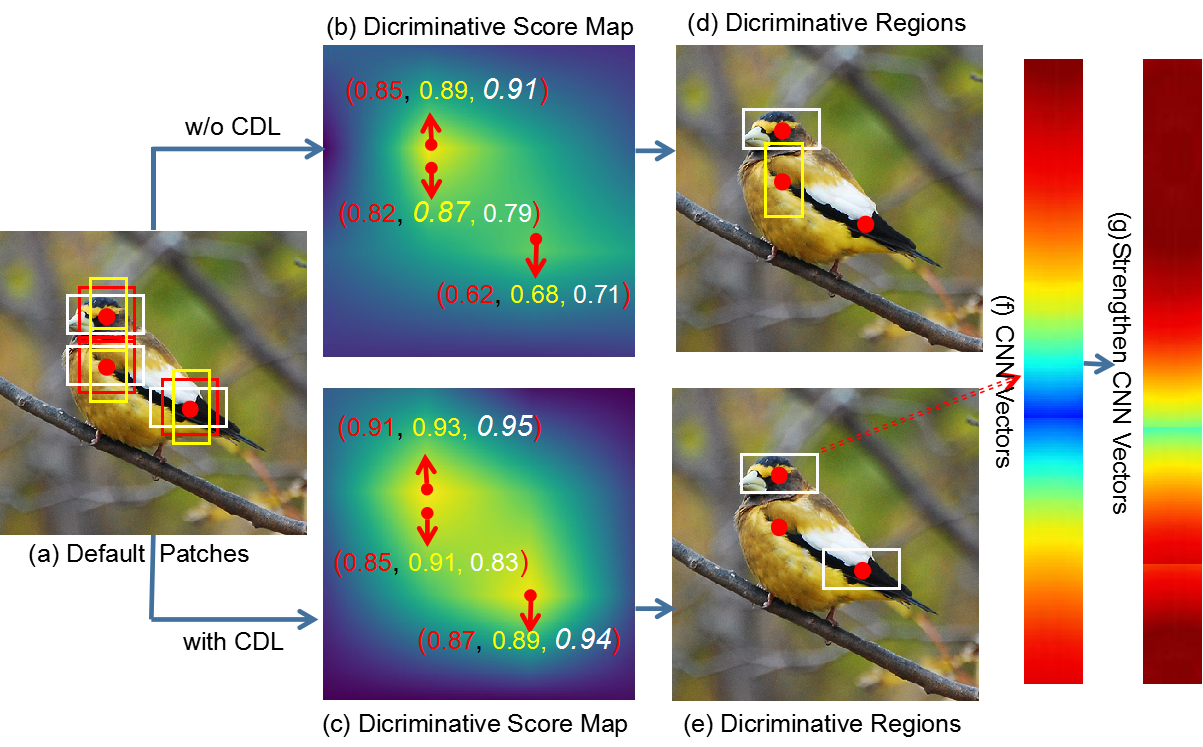
\includegraphics[width=0.6\textwidth]{docs/paperReading/CDL/summary.png}
    \end{figure}
    \begin{scriptsize}
        (b)(d)是没有相关性引导的判别学习,(c)(e)是有相关性引导的判别学习
        
        (f)是CNN的feature,(g)是挖掘相互依赖之后的feature
    \end{scriptsize}
\end{frame}



\begin{frame}{The framework of the Correlation-guided Discriminative Learning (CDL) model}
    \begin{wrapfigure}{l}{0.7\textwidth}    % 靠文字内容的左侧
        \centering
        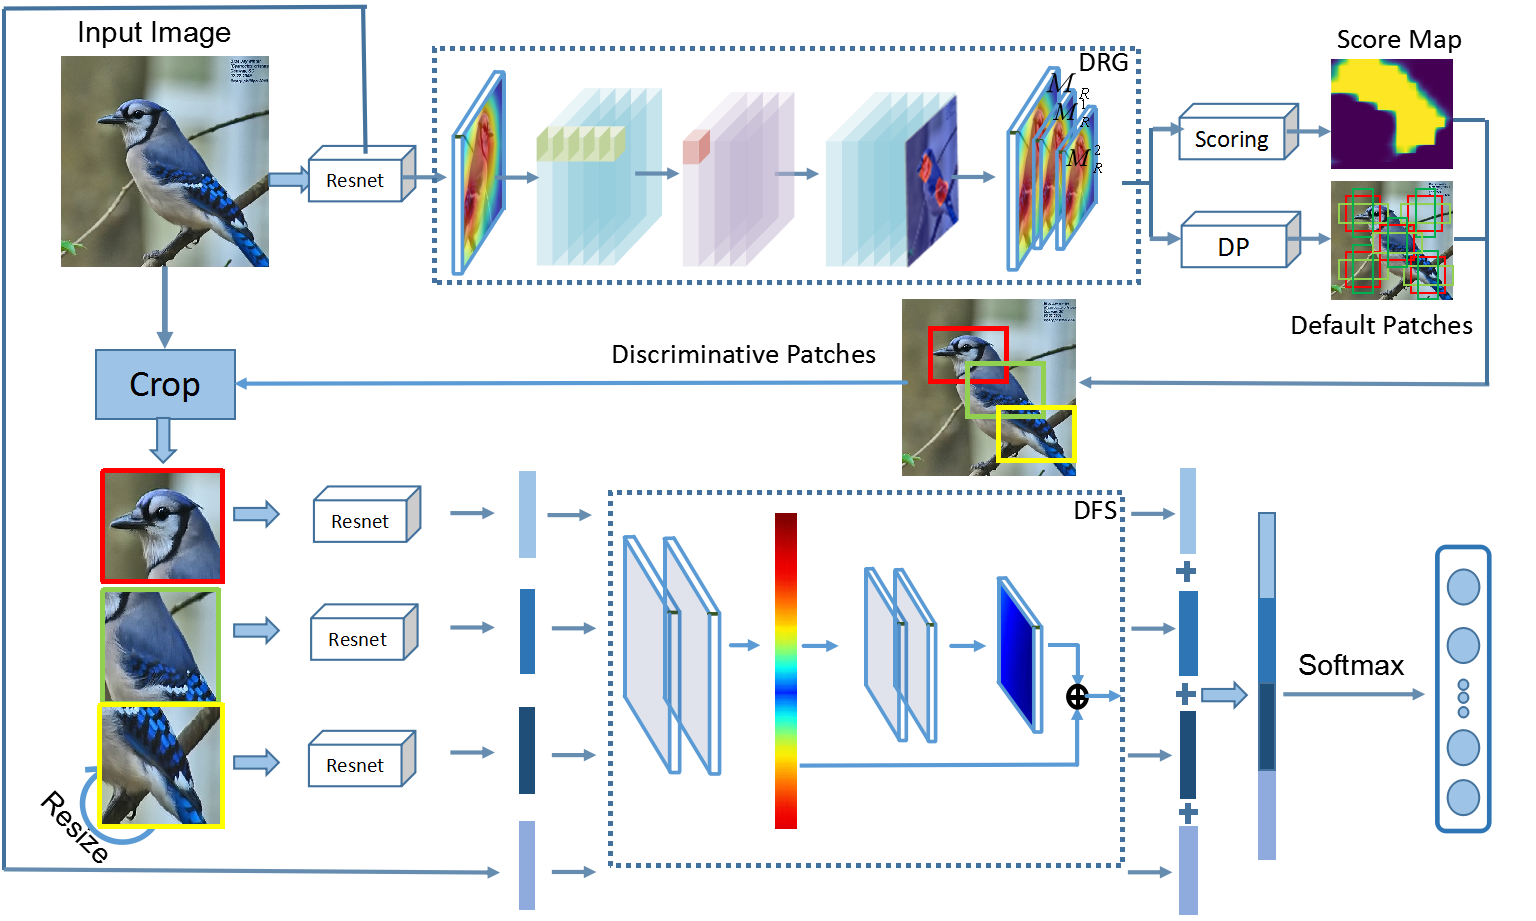
\includegraphics[width=0.6\textwidth]{docs/paperReading/CDL/framework.png}
        % \caption{\footnotesize framework of CDL}
    \end{wrapfigure}

    % 不能在任何列表环境中使用 wrapfigure,也不能在列表环境前后使用,除非两者之间有一空行或分段指令 \par。
    CDL model:
    \begin{scriptsize}
        \begin{itemize}
            \item \textbf{DGR} 判别区域分组子网络
            \item \textbf{Scoring} 评分网络
            \item \textbf{DP} 根据score map选择更具判别性的patch
            \item \textbf{Resize} 224*224
            \item \textbf{DFS}(discriminative feature strengthening) 判别性特征增强子网络
            \item concat the multiply feature
        \end{itemize}
    \end{scriptsize}    
\end{frame}


\begin{frame}{Discriminative Region Grouping(DRG)}
    \begin{multicols}{2}
        \begin{figure}
            \centering
            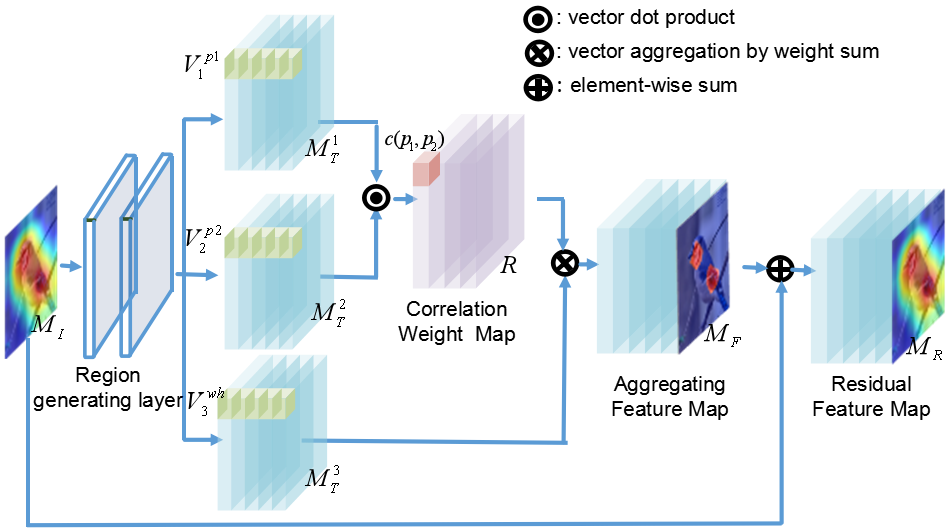
\includegraphics[width=0.52\textwidth]{docs/paperReading/CDL/dgr.png}
        \end{figure}
        
        DRG
        \begin{scriptsize}
            (Discriminative Region Grouping),学习两个区域的相关性系数,与原特征图加权后可以得到聚合特征图,最后通过残差学习将输入特征图的全局语义信息和局部细节信息进行整合,提取出有区别的小块
            \begin{enumerate}
                \item \textbf{region generating layer.}: 1*1 kernel的小区域检测器(small region detector)。
                \item \textbf{correlation layer.}
                \item \begin{equation}
                    R=softmax(V_1^{p_1}\cdot V_2^{p_2})
                \end{equation}
                \item \textbf{fusion(aggregating) layer.}
                \begin{equation}
                    M_F^{ij}=\sum_{w=1}^W\sum_{h=1}^H(V_3^{wh}\cdot R^{ijk}),k=(w-1)\times W+h
                \end{equation}
                \item \textbf{residual block.} $W_R=\alpha\cdot M_F+M_I$
            \end{enumerate}
        \end{scriptsize}
    \end{multicols}
        
\end{frame}

\begin{frame}{Picking Out Discriminative Patches} 
    \begin{multicols}{2}
        \begin{figure}
            \centering
            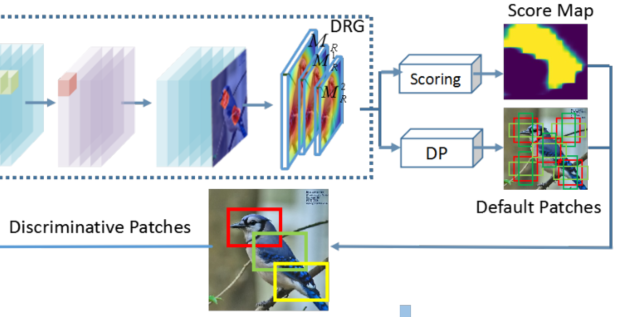
\includegraphics[width=0.35\textwidth]{docs/paperReading/CDL/dp.png}
        \end{figure}
        对残差模块生成的多尺度 $M_R^i(i=1,2,3)$ 计算 \textbf{discriminative probability maps} (Score Map) \footnote{$1\times 1$kernel+sigmoid} $S$,来表示判别区域对最终图像分类结果的影响。网络会选择top-N个个patch+区别的概率值$s_{ijk}$
        
        $p_{ijk}=tensor(t_x,t_y,t_w,t_h,s_{ijk})$
\end{multicols}
    
\end{frame}


\begin{frame}{Discriminative Feature Strengthening(DFS)}
    \begin{figure}
        \centering
        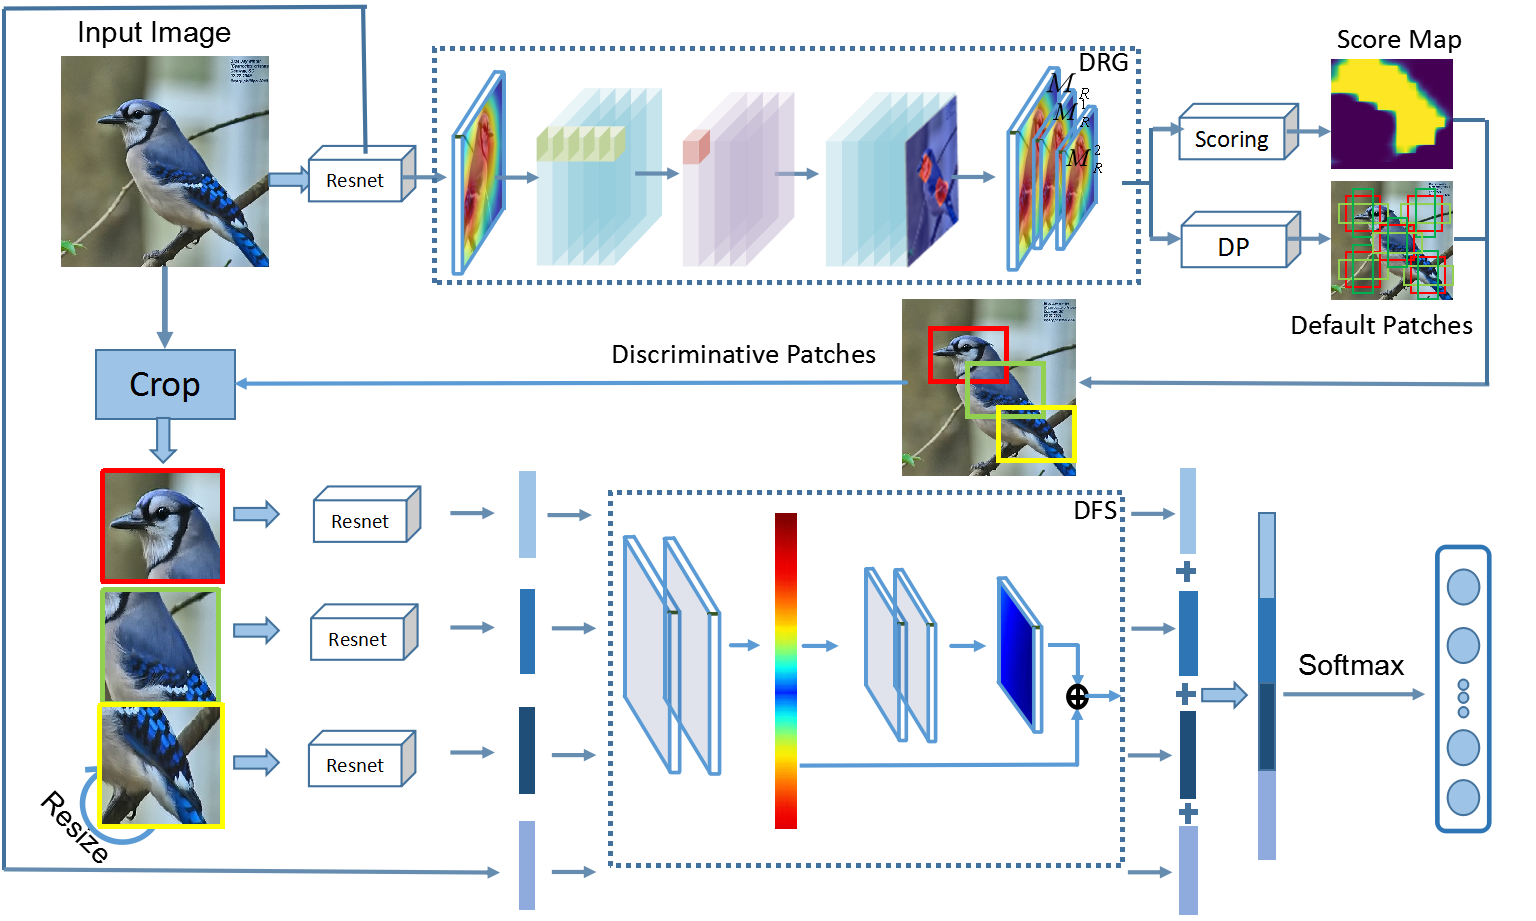
\includegraphics[width=0.6\textwidth]{docs/paperReading/CDL/framework.png}
        % \caption{\footnotesize framework of CDL}
    \end{figure}
    \textbf{DFS}(discriminative feature strengthening) 判别性特征增强子网络
\end{frame}
\begin{frame}{Discriminative Feature Strengthening(DFS)} 
    \begin{figure}
        \centering
        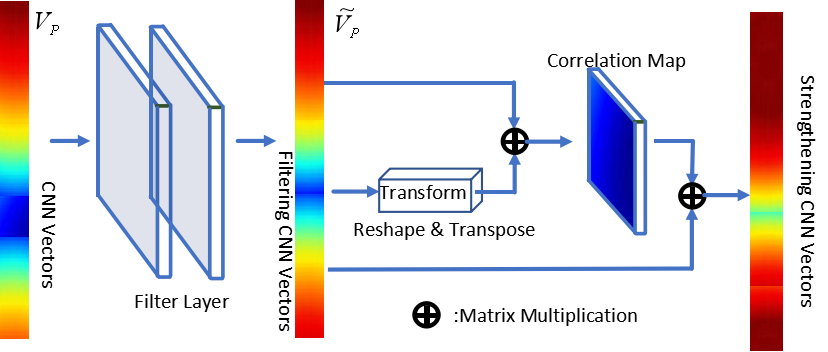
\includegraphics[width=0.5\textwidth]{docs/paperReading/CDL/dfs.png}
    \end{figure}
    \begin{scriptsize}
        \begin{enumerate}
            \item 过滤(filter layer)无用信息$\tilde{V_p}=ReLU(BN(W*V_p+b_p))$
            \item enhancement layer. $\tilde{S_E^{ij}}=softmax(S_E^{ij})=softmax(\tilde{V_pi}\cdot \tilde{V_pj}^T)$
            \item 经过增强的feature. $V=\tilde{V_p}\cdot \tilde{S_E}$
            \item 残差学习保证robustness. $\tilde{V}=\beta\cdot V+V_P$
        \end{enumerate}
    \end{scriptsize}
\end{frame}

\begin{frame}{Loss Function}
    \begin{scriptsize}
        \textbf{Multi-task loss} $\mathcal{L}$, 
        fine-grained classification loss$\mathcal{L}_{cls}$, 
        guided loss$\mathcal{L}_{gud}$, 
        correlation loss$\mathcal{L}_{rela}$, 
        rank loss $\mathcal{L}_{rank}$
        \begin{equation}
            \mathcal{L}=\mathcal{L}_{cls}
            +\lambda_1\cdot\mathcal{L}_{gud}
            +\lambda_2\cdot\mathcal{L}_{rela}
            +\lambda_3\cdot\mathcal{L}_{rank}
            \footnote{After many experiment verifications, set $\lambda_1=\lambda_2=\lambda_3=1$}
        \end{equation}
        
        \textbf{guided loss} $\mathcal{L}_{gud}$\footnote{$X$是原始图像,$C$是分类的置信度函数,选择的patch$P=\left\{P_1,P_2,...,P_N\right\}$和对应得分$S=\left\{S_1,S_2,...,S_N\right\}$}引导网络识别出更具判别性的区域。当所选区域的预测概率值低于整幅图像的预测概率值时,损失增加
        \begin{equation}
            \mathcal{L}_{gud}(X,P)=\sum_i^N max\left\{0,log{C(X)}-log{C(P_i)}\right\}
        \end{equation} 
        
        \textbf{correlation loss} $\mathcal{L}_{rela}$\footnote{$P_c$是所选择的特征的拼接}保证组合特征的预测概率大于单个特征的预测概率
        \begin{equation}
            \mathcal{L}_{rela}(P_c,P)=\sum_i^N max\left\{0,log{C(P_i)}-log{C(P_c)}\right\}
        \end{equation}
        
        \textbf{rank loss} $\mathcal{L}_{rank}$使得patch判别分数和最终分类概率一致,
        \begin{equation}
            \mathcal{L}_{rank}(S,P)=
            \sum_{log{C(P_i)}<log{C(P_j)}} (max\left\{0,(S_i-S_j)\right\})
        \end{equation}
    \end{scriptsize}
\end{frame}

\begin{frame}{Result:Quantitative Comparisons}
    \begin{wrapfigure}{l}{0.5\textwidth}    % 靠文字内容的左侧
        \centering
        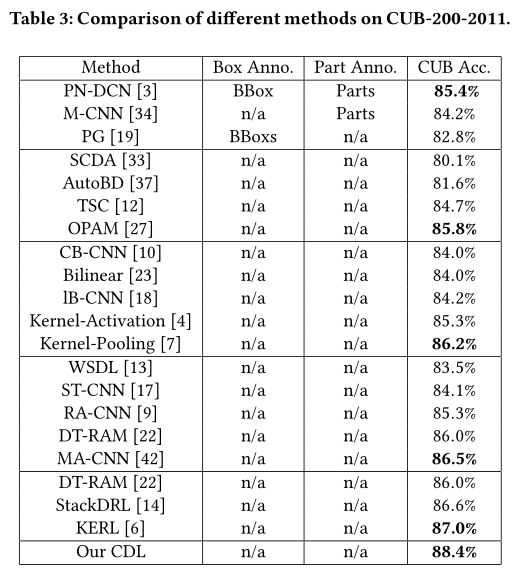
\includegraphics[width=0.35\textwidth]{docs/paperReading/CDL/comparison-1.png}        
    \end{wrapfigure}    
    \begin{scriptsize}
        \textbf{Accuracy Comparison.} \footnote{\textbf{Dataset}:Caltech-UCSD Bird-200-2011(CUB-200-2011)}        
        \begin{enumerate}
            \item supervised multi-stage methods
            \item weakly supervised multi-stage frameworks
            \item weakly supervised end-to-end feature encoding
            \item end-to-end localization-classification sub-networks
            \item other methods(reinforcement learning, knowledge representation)
            \item CDL.
        \end{enumerate}
        \textbf{Speed Comparison.}
        \begin{figure}
            \centering
            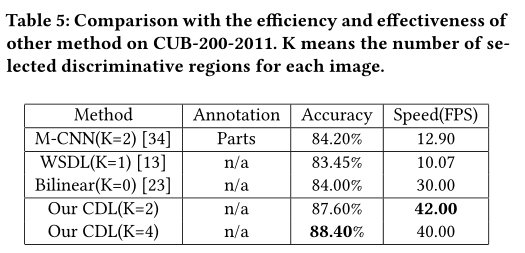
\includegraphics[width=0.35\textwidth]{docs/paperReading/CDL/comparison-2.png}
        \end{figure}
    \end{scriptsize}
\end{frame}


\begin{frame}{Result:Qualitative Analysis}
    \begin{multicols}{2}
        \begin{figure}
            \centering
            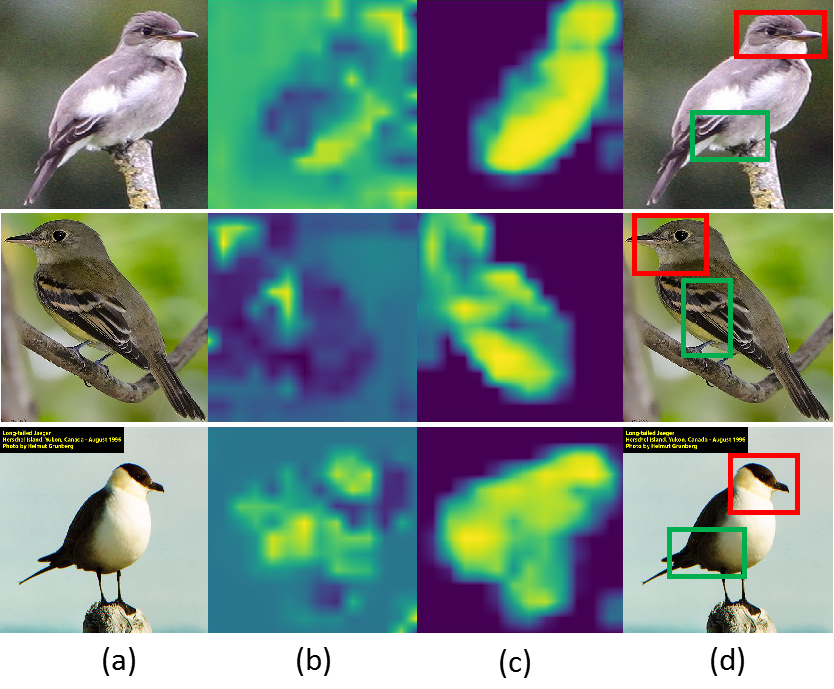
\includegraphics[width=0.32\textwidth]{docs/paperReading/CDL/result-2.png}
        \end{figure}
        \begin{scriptsize}
            判别性区域分组的可视化中间结果
            \begin{enumerate}
                \item \textbf{(a)}原始图像
                \item \textbf{(b)}相关性聚合的特征图$R^{ijk}$
                \item \textbf{(c)}残差特征图$M_R$
                \item \textbf{(d)}定位结果
            \end{enumerate}
        \end{scriptsize}  

        \begin{figure}
            \centering
            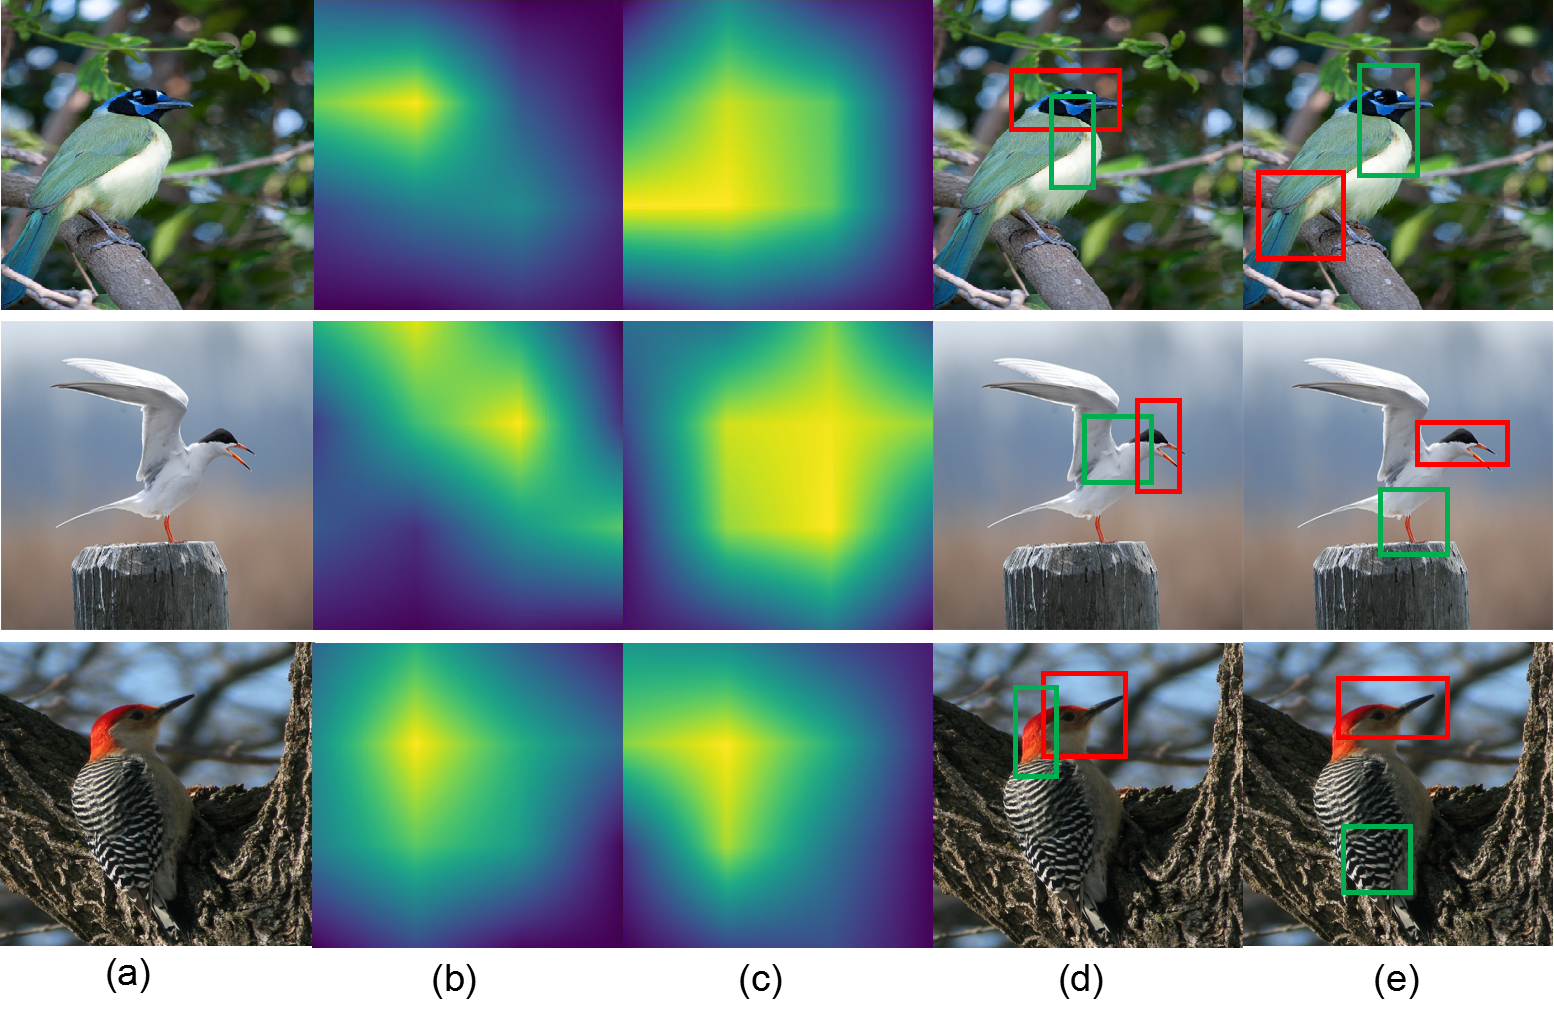
\includegraphics[width=0.4\textwidth]{docs/paperReading/CDL/result-3.png}
        \end{figure}
        \begin{scriptsize}
            区域间有无相关性的可视化定位结果
            \begin{enumerate}
                \item \textbf{(a)}原始图像
                \item \textbf{(b)(d)}无相关性判别的得分图、定位结果
                \item \textbf{(c)(e)}有相关性判别的得分图、定位结果
            \end{enumerate}
        \end{scriptsize}
    \end{multicols}
    
    
    
\end{frame}